\chapter{State of the art Survey}

This chapter introduces some of the technologies currently available that deal with anonymity and privacy. Some of the technologies are already commercially available and being used in the industry, while others are still in research phase. We will give a brief introduction for all of them and a brief idea of how they can be used.

\section{Definitions and Common Terminology}
Below are the main terminologies and definitions used in this thesis. Some of the terms are taken from \cite{goldberg2000pseudonymous}:
\begin{itemize}
\item\textbf{Privacy :}
It is the ability of an individual to control the distribution of information about himself. An individual should be able to choose which information about him should remain secret and which information can be revealed.
\item\textbf{Anonymity\cite{Anonymity} :}
It refers to the ability of a user to not give any information about him at all to the system. It is the state of not being identifiable in the system. An anonymous system doesn't have any identity of the user.
\item\textbf{Pseudonym\cite{Pseudonyms} :}
It is a name given to the user in pseudonymous systems. This name is given to hide the real identity of the user from the system. The system only knows the user by his pseudonym.
\item\textbf{User :}
It is the end user of the system. It is the person who will go online and get the services. In our system, most of the time, we refer to user as the employee of the company, who is accessing the services of the bank.
\item\textbf{Bank :}
It is the financial institution which provides online financial services to the user. In our system, we refer to Nykredit as the bank.
\item\textbf{Third party :}
A third party or trusted third party is the entity which is neither the bank or the user in the system. A third party provides different services to banks or users and hence reduces the burden on them to setup all the infrastructure by themselves. In our system, Signicat is referred to as the third party.
\item\textbf{Service :}
It is something that is provided to the user online by a system. It may include the ability to login, check his account balance, upload pictures, share spreadhseets etc.
\item\textbf{Unlinkability :}
It is the privacy property where it is not possible to link 2 different entities to each other even though they are the same. 
e.g. not to be able to link 2 different sessions by the same user in the system.
\item\textbf{Revocation :}
It is the property where a user credential is revoked by the user or some other authority. After revocation, this credential cannot be used for anything.
\item\textbf{Partial Information Disclosure :}
It is the ability of a user to only disclose some partial information about himself to the system. e.g. a user might just want to disclose his last name to the system but not his full name.
\item\textbf{Legal Requirement :}
It is something that is required by law. e.g. it may be required by law that the bank logs all the customer data. Also sometimes in case of suspicious transactions the bank may be required legally to give the user identity to the relevant authorities.
\item\textbf{Conditional Anonymity Removal :}
It is the ability of the system to remove anonymity of the user if some conditions that were set before are met. This is mainly used for escrow purposes.
\item\textbf{Verifiable Encrytion{\cite{VE}} :}
It is a type of encryption in which encrypted data can be verified i.e. someone who doesn't know the actual data can verify that the encrypted data is the same as claimed by the person who encrypted it. e.g. if the person who is encrypting the data has to encrypt his key in it, it can be verified that he has encrypted his real key and not some garbage value.
\item\textbf{Zero Knowledge Proof\cite{ZK}\cite{feige1988zero} :}
It is a type of proof where the prover is able to convince the verifier that a statement is valid without giving any other information about the statement except that it is valid. e.g. if a user has to prove that he has the private key to a particular public key, he can prove it without giving away any other information about his private key.
\end{itemize}
\section{Technologies}
After getting the requirements and based on our terminology we looked at the current technologies. We came out with a map as in figure \ref{fig:Technologies}. Basically we divided our type of technologies in 4 different types, depending on the functions:
\begin{enumerate}
	\item Secure Multi-Party Computing
	\item Escrow Technologies
	\item Identity Management Systems
	\item Zero Knowledge Technologies
\end{enumerate}
\begin{figure}[h]
	\centering
	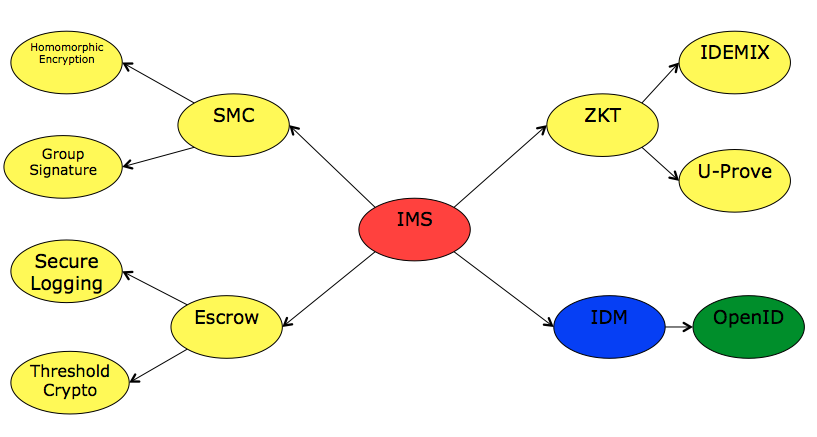
\includegraphics[width=\textwidth]{figures/Technologies}
	\caption{Technology Overview}
	\label{fig:Technologies}
\end{figure}
\section{Secure Multi-Party Computing}
These technologies are the ones which involve multiple parties to do computations\cite{goldreich1998secure}. It is a subfield of cryptography which involves multiple parties getting an input and compute a joint function on them while keeping these inputs private. We basically looked at 2 technologies of interest here:
\subsection{Homomorphic Encryption}
\textit{Homomorphic encryption}\cite{rappe2005homomorphic} is a type of encryption where certain arithmetic operations can be performed on the \textit{ciphertext} so that when the resultant ciphertext is decrypted, the decrypted text is the same as if the operations were performed on the \cite{plaintext}. This is a new field of cryptography and is very useful where we need some parties to perform such operations without revealing the underlying data to those parties. Homomorphic encryption is also useful for the chaining of different services without exposing data to any of those services.
\subsection{Group Signature}
A \textit{group signature}\cite{ateniese2000practical} is a scheme which allows a member of the group to sign the message on behalf of the group but anonymously. To outsiders the message has been signed by someone from the group but the exact identity of the person is now known. Also if the same member signs 2 different messages; it is not possible to know if the message is signed by the same member or 2 different members. There is a notion of \textit{group manager} in these scheme. Group manager is someone who manages the membership to the group. He can add/remove members from the group, find out who actually signed the message from the group. This scheme is useful where the only thing that needs to be validated is that a certain person is part of the group, but his real identity is not required.
\section{Escrow Technologies}
\textit{Escrow technologies} are those which are helpful in escrow purposes i.e. getting real data/identity later on in time from encrypted data if needed. We look at the 2 following technologies:
\subsection{Secure Logging}
\textit{Secure logging}\cite{accorsi2006relationship} is the process of saving the data in a secure manner, as saved data is really crucial and vulnerable to attacks. We need to make sure that the data is saved securely and its integrity is protected. This can be done in several ways. One way is to encrypt all the logs while storing them so that even if someone gets hold of the logs, they can't use them without having access to the decryption key. Another way is to store logs at a third party after encrypting them. For escrow purposes these logs can be decrypted later on with the decryption key.
\subsection{Threshold Cryptography}
\textit{Threshold cryptography}\cite{DBLP:conf/acisp/DamgardJ03} is a field of public key cryptography where in order to decrypt an encrypted message, several parties must cooperate in the decryption. This message is encrypted using a \textit{public key} and the corresponding \textit{private key} is shared among different parties who will participate in the decryption process i.e. multiple parties hold the private key for a single public key. There is a term known as \textit{threshold}, and if there are \textit{n} parties who share the private key and at least \textit{t} parties which are required to decrypt the message such system is called \textit{(t,n)} threshold cryptosystem. Threshold cryptosystem is useful in escrow purposes where a minimum number of parties are required to decrypt the ciphertext in order to get the plaintext.

\section{Identity Management Systems}
These are traditional identity management systems. For our purposes we look at the \textit{OpenID}\cite{recordon2006openid} system.
\subsection{OpenID}
OpenID is an open and decentralized protocol, which can be used to authenticate with different co-operating sites with the use of a third party service. It has the notion of a \textit{relying party} and \textit{OpenID identity provider}.
\begin{itemize}
\item \textbf{OpenID Identity Provider :} It is the service, which actually provides authentication services. End user registers at OpenID identity provider to get his OpenID identity.
\item \textbf{Relying Party :} It is the website which user wants to authenticate to and which rely on the OpenID identity provider to provide authentication.
\end{itemize}
In addition to this an extension called \textit{OpenID attribute exchange}\cite{hardt2007openid} helps facilitate the transfer of user attributes from the identity provider to the relying party.
\begin{itemize}
\item The user goes to the relying party service page.
\item The service page presents different OpenID providers to login to the service.
\item The user chooses the provider with whom he has registered his OpenID.
\item The relying party redirects the user to the OpenID provider url so that the user can authenticate.
\item The user can be authenticated by the method provided by the OpenID provider.
\item The OpenID provider asks the user to get his permission to share the attributes with the relying party.
\item After the user gives his consent, he is redirected to the relying party website with the user credentials.
\item The relying party can verify the credentials and then login the user to the service.
\end{itemize}
\section{Zero Knowledge Technologies}
These are the technologies which use the concept of zero knowledge\cite{ZK} i.e. proving knowledge about something without divulging the information. For our purpose we focus on 2 main technologies – \textit{IDEMIX}\cite{1_zurich_ibm_com_2015} and \textit{U-Prove}\cite{3_research_microsoft_com_2015}, which are based on the concept of zero knowledge\cite{ZK} and verifiable encryption\cite{VE}. They both have a lot in common and have been studied a lot. 
\subsection{IDEMIX}
IDEMIX\cite{camenisch2001efficient}\cite{camenisch2002design}is a digital credential technology by IBM. It relies on anonymous credentials known as IDEMIX tokens. It is based on Camenisch-Lysyanskaya (CL) signature scheme\cite{camenisch2003signature} which provides efficient zero-knowledge proofs. IDEMIX  has different entities in the system:
\begin{itemize}
	\item \textbf{User :} It is basically the entity who is proving his identity in the system.
	\item \textbf{Verifier :} It is the entity that verifies the identity of the prover.
	\item \textbf{Issuer :} It is the entity that issues the credentials to the prover to prove his identity
	\item \textbf{Inspector :} It is the entity which, in case of discrepancy or legal requirement, can actually come and get the real identity of the prover.
\end{itemize}
\begin{figure}[h]
	\centering
	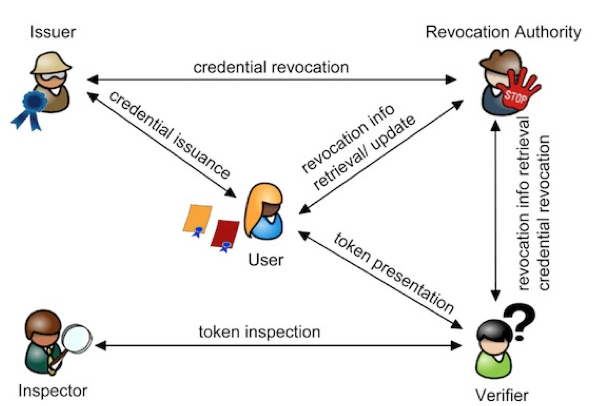
\includegraphics[width=\textwidth]{figures/Roles}
	\begin{minipage}{\textwidth}
		\footnotesize
		\emph{Source: https://github.com/p2abcengine/p2abcengine/wiki/Concepts-and-features}
	\end{minipage}
	\caption{IDEMIX Roles}
	\label{fig:Roles}
\end{figure}
Figure \ref{fig:Roles} shows these roles in detail.

For IDEMIX we need \textit{computing devices} that work on behalf of each entity in the system.
\subsubsection{IDEMIX Credential}
An IDEMIX credential is a \textit{CL Signature}\cite{camenisch2003signature} by issuer on the user's private key and on the attribute values. A user has independent public keys or pseudonyms for the same private key. These pseudonyms are IDEMIX tokens which are then used by the user to prove his identity to the different verifiers. IDEMIX has been studied a lot and many EU projects on anonymous credentials are based on it e.g. FutureID\cite{rossnagel2012futureid}, ABC4Trust\cite{sabouri2012attribute} etc. An example of an IDEMIX credentials is shown in figure \ref{fig:Credential}.
\begin{figure}[h]
	\centering
	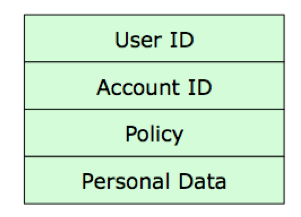
\includegraphics[width=170pt]{figures/Credential}
	\caption{IDEMIX Credential}
	\label{fig:Credential}
\end{figure}
\subsubsection{Issuance}
The first step is the credential issuance. It involves the following steps:
\begin{itemize}
	\item The user sends a credential request to the issuer.
	\item The issuer presents the \textit{issuance policy} specifying:
	\begin{itemize}
		\item What attributes to present.
		\item Which pseudonym/existing credentials to present.
	\end{itemize}
	\item The issuer also present a \textit{credential template} specifying:
	\begin{itemize}
		\item Which attributes of the new credentials will be generated at random.
		\item and which attributes will be carried over from existing credential or pseudonym.
	\end{itemize}
	\item The user then presents the issuance token satisfying the issuance policy.
	\item Then multi-round cryptographic protocol ensues, at end of which, the user gets the IDEMIX credential.
\end{itemize}
\subsubsection{Presentation}
The next step is to present the IDEMIX token for authentication to the verifier. It consists of the following steps:
\begin{itemize}
	\item The user gets the presentation policy from the verifier which specifies:
	\begin{itemize}
		\item Which credentials the user must present.
		\item What information the user should reveal from these credentials.
	\end{itemize}
	\item The user generates a presentation token in accordance with the presentation policy revealing only the necessary attributes. 
	\item The user presents this presentation token to the verifier.
	\item The verifier can then verify the attributes from the presentation token presented by the user.
\end{itemize}
\subsubsection{ID Escrow}
IDEMIX provides the ID escrow ability in case it is required. The steps below need to be followed for ID escrow purposes in IDEMIX:
\begin{itemize}
	\item The presentation policy can have the following optional specifications for the purpose of ID Escrow:
	\begin{itemize}
		\item Public keys of the inspectors.
		\item Attribute values to be encrypted using the keys.
		\item Inspection conditions under which these attributes can be revealed.
	\end{itemize}
	\item The user can prove that he has put these values in the presentation token with verifiable encryption\cite{camenisch2003practical} to the verifier.
	\item Once the token in presented, the inspection conditions are fixed and cannot be changed. 
	\item In case of some discrepancy or legal requirement, an inspector can come and get the identity of the user from the token.
	
	A visual representation of creating an IDEMIX presentation token from the IDEMIX credential can be seen in figure \ref{fig:Token}.
\end{itemize}
\begin{figure}[h]
	\centering
	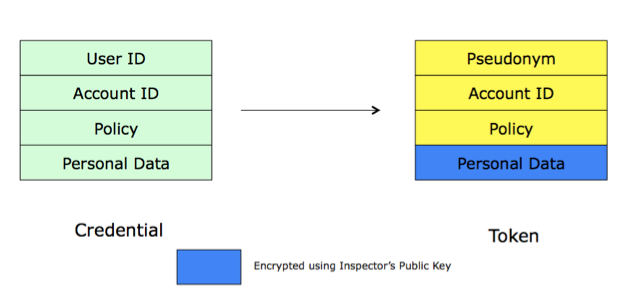
\includegraphics[width=\textwidth]{figures/Token}
	\caption{IDEMIX Presentation Token}
	\label{fig:Token}
\end{figure}

\subsection{U-Prove}
U-Prove is a digital credential technology by Microsoft\cite{paquin2013u}\cite{paquin2011u}. It relies on anonymous credentials known as U-Prove tokens. It provides users a way to minimaly disclose their personal information while interacting with different online services. U-prove have different entities in the system
\begin{itemize}
	\item \textbf{Prover :} It is basically the entity, which is proving his identity in the system.
	\item \textbf{Verifier :} It is the entity, which verifies the identity of the prover.
	\item \textbf{Issuer :} It is the entity, which issues the credentials to the prover to prove his identity
	\item \textbf{Auditor :} It is the entity, which in case of discrepancy or legal requirement , can actually come and get the real identity of the prover.
\end{itemize}
For U-Prove we need computing devices which work on behalf of each entity in the system.
\subsubsection{U-Prove Token}
A U-Prove token is basically cryptographically protected information of any kind e.g. attributes. These are issued by an issuer to the prover by \textit{issuance protocol}. These tokens are then presented by the prover to the verifier. Issuance and presentation of U-Prove tokens is unlinkable.
\subsubsection{Issuance}
The first step is the credential issuance. It involves the following steps:
\begin{itemize}
	\item The prover invokes U-Prove issuance protocol.
	\item The prover provides the attributes to be encoded.
	\begin{itemize}
	\item Using the \textit{Collaborative Issuance}\cite{paquin2014u} property user can make sure that the issuer doesn’t actually know the attributes.
\end{itemize}
	\item Then multi-round cryptographic protocol ensues at end of which the user get the U-Prove token from the issuer.
\end{itemize}
\subsubsection{Presentation}
The next step is to present the U-Prove token for authentication to the verifier. It consists of the following steps:
\begin{itemize}
	\item The prover invokes the U-Prove \textit{presentation protocol}.
	\item The user generates a presentation token in accordance with the presentation policy revealing only the necessary attributes. 
	\item The user presents this presentation token to the verifier.
	\item The verifier can then verify the attributes from the token presented by the user.
\end{itemize}
It must be noted that a revocation check can be added if needed before verifying the token.
\subsubsection{ID Escrow}
ID Escrow in U-Prove is actually an extension\cite{zaverucha2013u} to existing U-Prove technology. It uses a type of ElGamal encryption which is verifiable.
\begin{itemize}
	\item  During the presentation protocol, the prover proves that his ID is encrypted in the token by the use of verifiable encryption\cite{VE} technology.
	\item De-anonymization cannot be done by the verifier or the issuer.
	\item A special entity called Auditor is responsible for de-anonymization in case of some discrepancy or legal requirement
	\item Threshold cryptography\cite{DBLP:conf/acisp/DamgardJ03} can be used and the decryption key can be split among multiple auditors.
\end{itemize}

All these different technologies provide different \textit{levels of anonymization}\cite{goldberg2000pseudonymous} in the system. Some of them are easy to integrate in existing technology, while others are still not mature enough. From now on we focus mainly on 2 technologies:
\begin{itemize}
	\item OpenID
	\item IDEMIX
\end{itemize}